\documentclass[12pt]{article}
\usepackage{graphicx} 
\usepackage{caption}
\usepackage{float}

\usepackage[utf8]{inputenc}
\usepackage[romanian]{babel}
\usepackage[T1]{fontenc}
\usepackage{indentfirst} % for automatic indentation

\usepackage{hyperref}
\hypersetup{
    colorlinks=true,
    linkcolor=black,
    filecolor=magenta,      
    urlcolor=cyan,
}

% For extended customization of titles
\usepackage{titlesec}
% For setting document margins
\usepackage{geometry}
% For enhanced color support
\usepackage{xcolor}

% Set document margins
\geometry{left=2.5cm, right=2.5cm, top=2.5cm, bottom=2.5cm}

% Adjusting paragraph indents and spacing
\usepackage{parskip}
\setlength{\parindent}{1em}
\setlength{\parskip}{1em} % Adjust space between paragraphs

% Customizing section titles
\titleformat{\section}
  {\normalfont\Large\bfseries}{\thesection}{1em}{}

% Customizing subsection titles
\titleformat{\subsection}
  {\normalfont\large\bfseries}{\thesubsection}{1em}{}

% Customizing subsubsection titles
\titleformat{\subsubsection}
  {\normalfont\normalsize\bfseries}{\thesubsubsection}{1em}{}

\begin{document}

\begin{titlepage}

    \begin{minipage}{0.6\textwidth}
        
\includegraphics[width=7cm]{logo_ro-RO.png}
    \end{minipage}
    \begin{minipage}{0.3\textwidth}
        \center
        {Programul de studii: \\ Informatic\u{a} Aplicat\u{a}}
    \end{minipage}
    
    \vspace*{5 cm} 

    \begin{center}
            {\Large \textbf{Lucrare de licență \\ Detectia numerelor de inmatriculare}}\\[2 cm]        
    \end{center}

    \vspace*{2 cm} 
    
    {\raggedright \normalsize \textbf{Absolvent:} Doloiu Mihai Alexandru \\ \textbf{Coordonator științific}: Lect. Dr. Vlad Monescu}
    
    \vspace*{\fill} 
    \begin{center}
        {\Large \centering \textbf{Brasov, 2024}}
    \end{center}
\end{titlepage}

\tableofcontents

\listoffigures

\newpage

\section{Introducere}

\subsection{Scopul lucrării}

\subsection{Motivația alegerii temei}

\subsection{Descrierea capitolelor}
%\begin{itemize}
%    \item \textbf{Medii si concepte de programare:} Acest capitol
%\end{itemize}

\section{Medii si concepte de programare}

\subsection{Limbajul de programare C++}

Inițial denumit "C cu clase", C++ este un limbaj de programare de nivel \^{i}nalt, ce este considerat a fi o extensie și o \^{i}mbunatațire a limbajului C. Acesta p\u{a}streaz\u{a} toate caracteristicile limbajului C și aduce concepte specifice program\u{a}rii orientate pe obiecte, precum clase, obiecte, incapsulare, moștenire, polimorfism, gestionare de excepții și multe altele. Fiind un limbaj de programare orientat pe obiecte, accentul este pus mai mult pe "obiecte" și nu pe manipularea lor. Pe l\^{a}ng\u{a} caracteristica menționat\u{a} anterior, C++ mai dispune și de alte caracteristici la care se num\u{a}r\u{a}: 

\begin{itemize}
    \item Viteza de compilare - deoarece C++ este un limbaj compilat, \^{i}nsemn\u{a}nd c\u{a} codul surs\u{a} al acestuia este tradus direct \^{i}n cod mașin\u{a}, programul rezultat beneficiaz\u{a} de performanțe superioare \^{i}n comparație cu alte limbaje de programare.
    \item Suport pentru pointeri - deși \^{i}n ziua de ast\u{a}zi acest lucru este indisponibil \^{i}n multe alte limbaje de programare, C++ ofer\u{a} o modalitate de a manipula și gestiona direct memoria cu ajutorul pointerilor.
    \item Portabilitate - fiind unul dintre cele mai utilizate limbaje din lume, codul C++ poate fi scris astfel \^{i}nc\^{a}t s\u{a} ruleze pe mai multe platforme hardware și sisteme de operare.
    
\end{itemize}
% cplusplus.com/info/description (ro/en)

Av\^{a}nd \^{i}n vedere caracteristicile menționate, acestea contribuie la eficiența și adaptabilitatea sa, facilit\^{a}nd dezvoltarea aplicațiilor pe diverse platforme și \^{i}n diverse contexte. Astfel, fiind unul dintre cele mai importante si puternice limbaje de programare, am decis ca implementarea codului surs\u{a} al aplicației pentru detectarea și recunoașterea numerelor de \^{i}nmatriculare, dar și pentru gestionarea bazei de date a acesteia, s\u{a} fie realizat\u{a} \^{i}n C++.

\subsection{Limbajul de programare Java}

Java, la fel ca și C++, este tot un limbaj de programare de nivel \^{i}nalt, orientat pe obiecte, dar bazat pe clase, unde fiecare fișier este de fapt o clas\u{a}. A fost dezvoltat pentru a oferi portabilitate, performanț\u{a} și securitate, fiind creat cu scopul de a fi independent de platform\u{a}, eficient și simplu. At\^{a}t Java, c\^{a}t și C++, prezint\u{a} numeroase similarit\u{a}ți din punct de vedere al sintaxei limbajului, ins\u{a} limbajul Java este considerat a fi mai ușor de folosit. Printre principalele caracteristici ale limbajului Java se num\u{a}r\u{a}:

\begin{itemize}
    \item Programarea orientat\u{a} pe obiecte - Java, la fel ca și C++, dispune de conceptele specifice program\u{a}rii orientate pe obiecte, \^{i}mbun\u{a}t\u{a}țiind practicitatea limbajului de programare prin oferirea unei modalitați mai eficiente de structurare a codului, promov\^{a}nd reutilizarea, flexibilitatea și modularitatea.
    \item Independent de platform\u{a} - programele create \^{i}n Java pot fi rulate pe orice platform\u{a} hardware și sistem de operare datorit\u{a} faptului c\u{a} codul surs\u{a} este tradus \^{i}ntr-un format intermediar numit "Java Bytecode" care permite rularea programului oriunde se dispune de o masin\u{a} virtuala Java instalat\u{a} (\emph{JVM}\footnote{Java Virtual Machine - Mașin\u{a} virtual\u{a} Java}). JVM-ul \^{i}ncarc\u{a}, verific\u{a} și execut\u{a} Java Bytecode-ul, asigur\^{a}nd totodat\u{a} gestionarea memoriei, gestionarea excepțiilor, etc.
    \item Securitate - asupra securit\u{a}ții s-a pus un accent deosebit, fiind asigurat\u{a} prin diverse mecanisme, precum Sandboxing, care const\u{a} \^{i}n izolarea resurselor periculoase ale sistemului de operare prin rularea aplicației Java \^{i}ntr-un mediu controlat. Un alt mecanism este Garbage Collection, care previne scurgerile de memorie si dep\u{a}șirile de buffer.
\end{itemize}

\^{I}n prezent, Java este utilizat \^{i}n diverse aplicații și site-uri web, datorit\u{a} numeroaselor avantaje pe care le ofer\u{a}. Pentru site-ul web prezentat \^{i}n aceast\u{a} lucrare, implementarea acestuia va fi realizat\u{a} cu ajutorul limbajului de programare Java și a \emph{framework-ului}\footnote{Framework - set de biblioteci, unelte și convenții de programare care ofer\u{a} o infrastructur\u{a} pentru dezvoltarea rapid\u{a} și eficient\u{a} a aplicațiilor.} Spring.

Prin urmare, limbajul de programare Java se remarc\u{a} prin portabilitate, securitate și performanț\u{a}. Datorit\u{a} implement\u{a}rii \^{i}n mod robust a conceptelor fundamentale ale program\u{a}rii orientate pe obiect, se faciliteaz\u{a} crearea de cod bine structurat și ușor de \^{i}ntreținut.

\subsection{Rețele neurale artificiale}

Salut

\subsection{Rețele neurale convoluționale}

Salut
\subsection{Biblioteca OpenCV}

\emph{OpenCV}\footnote{OpenCV - Open Source Computer Vision Library.} este o bibliotec\u{a} open-source specializat\u{a} \^{i}n vedere computerizat\u{a}, procesarea imaginilor și \^{i}nv\u{a}țare automat\u{a}, dețin\^{a}nd peste 2500 de algoritmi ce pot fi utilizați \^{i}n diverse aplicații, precum recunoașterea facial\u{a}, detectarea obiectelor, analiza medical\u{a}. Aceasta a fost scris\u{a} \^{i}n limbajul de programare C++, ins\u{a} este compatibil\u{a} și cu alte limbaje de programare, inclusiv C++, Python, Java și Matlab.

Pentru procesarea de imagini, OpenCV ofer\u{a} o gam\u{a} variat\u{a} de funcții pentru manipularea imaginilor, precum conversia de la un spațiu de culoare la altul, ajustarea luminii și a contrastului, transform\u{a}ri geometrice, filtrare și altele. De asemenea, \^{i}n cadrul bibliotecii, exist\u{a} un modul numit OpenCV \emph{DNN}\footnote{DNN - Deep Neural Networks.}, dedicat utiliz\u{a}rii și implement\u{a}rii DNN-urilor \^{i}n aplicații de computer vision. Ofer\u{a} funcționalit\u{a}ți puternice \^{i}n implementarea inferenței modelelor DNN și suporta integrarea cu diferite framework-uri, precum TensorFlow, Caffe, Yolo, Darknet și altele.


\^{I}n proiectul C++, pentru detecția și recunoașterea numerelor de \^{i}nmatriculare ale mașinilor, s-a utilizat versiunea 4.8.0 de OpenCV. Biblioteca a fost utilizat\u{a} de la inceputul proiectului, \^{i}n timpul detect\u{a}rii placuței de \^{i}nmatriculare și a literelor de pe aceasta, unde s-au folosit algoritmii adecvați, p\^{a}n\u{a} la final, la recunoașterea caracterelor, unde s-a folosit un set de date ce conține toate caracterele de pe placuțele din Romania și s-a realizat template matching.

\subsection{Biblioteca YOLOv5}

\emph{YOLOv5}\footnote{YOLOv5 - You Only Look Once, versiunea 5.}, dezvoltat\u{a} de c\u{a}tre echipa Ultralytics, este o bibliotec\u{a} de Deep Learning și un framework pentru detecția diferitelor obiecte \^{i}n imagini și videouri. Ca structur\u{a}, se bazeaz\u{a} pe o abordare de tip "You Only Look Once", \^{i}nsemn\^{a}nd c\u{a} \^{i}n loc ca procesul de detecție s\u{a} fie \^{i}mp\u{a}rțit pe etape separate, cum ar fi detectarea, clasificarea și localizarea, acesta este tratat ca o singur\u{a} rețea neural\u{a}, abordare ce permite furnizarea predicțiilor \^{i}n timp real. Astfel, biblioteca YOLO este cunoscut\u{a} pentru eficiența sa. 

Biblioteca permite utilizatorilor s\u{a} antreneze modele folosind seturi de date proprii, folosind una dintre arhitecturile variate pe care biblioteca le furnizeaz\u{a}, cum ar fi YOLOv5s (Small), YOLOv5m (Medium), YOLOv5l (Large),  și realizarea inferenței (detecție de obiecte) pe imagini noi. 

\^{I}n proiectul dezvoltat pentru aceasta lucrare de diplom\u{a}, detecția placuțelor de \^{i}nmatriculare se poate realiza, la alegerea utilizatorului, at\^{a}t prin folosirea algoritmilor de procesare de imagini din OpenCV, c\^{a}t și prin folosirea unui model antrenat cu ajutorul acestei biblioteci.

\subsection{Framework-ul Qt}
%About qt
Qt este un framework utilizat pentru crearea de aplicații cross-platform, precum serverele, care ruleaz\u{a} pe diverse platforme software și hardware, cum ar fi Windows, Linux, OS X, Android, iOS, și altele. Preprocesorul \emph{MOC}\footnote{MOC - Meta-Object Compiler.} extinde limbajul C++ prin ad\u{a}ugarea de noi caracteristici necesare \^{i}n dezvoltarea aplicațiilor cu interfaț\u{a} grafic\u{a}, cum ar fi semnalele si sloturile. Exist\u{a} numeroase aplicații populare cu interfaț\u{a} grafic\u{a} realizate cu ajutorul framework-ului Qt și folosite de milioane de utilizatori din \^{i}ntreaga lume, printre care se num\u{a}r\u{a} Skype, Google Earth și browser-ul Opera.

Proiectarea și crearea de \emph{GUI}\footnote{GUI - Graphical User Interface} se realizeaza cu ajutorul uneltei grafice incluse in framework, Qt Desginer. Elementele grafice sunt atașate codului prin folosirea mecanismului de sloturi și a semnalelor Qt. Qt Designer genereaz\u{a} automat codul surs\u{a} asociat cu interfața, odat\u{a} ce aceasta este proiectat\u{a}. Acest lucru elimin\u{a} nevoia programatorilor de a scrie manual codul pentru fiecare element din interfaț\u{a}, economisind timp și evit\^{a}nd potențialele erori. Proiectarea interfețelor grafice ale aplicațiilor se realizeaza foarte ușor, av\^{a}nd posibilitatea ad\u{a}ug\u{a}rii si configur\u{a}rii a diferitelor elemente GUI, cum ar fi butoanele, etichetele, textbox-uri și altele, utiliz\^{a}nd pur și simplu drag-and-drop. Utilizarea Qt Designer implic\u{a} patru etape de baz\u{a}:
\begin{itemize}
    \item Alegerea propriei interfețe și a obiectelor dorite;
    \item Așezarea obiectelor pe interfața;
    \item Conectarea semnalelor la sloturile corespunz\u{a}toare;
    \item Vizualizarea interfeței.
\end{itemize}

Pentru realizarea interfeței grafice a aplicației principale, responsabil\u{a} pentru detecția și recunoașterea automat\u{a} a numerelor de \^{i}nmatriculare ale mașiniilor, s-a folosit framework-ul Qt. Meniul acesteia ofer\u{a} utilizatorului o metod\u{a} ușoar\u{a} și intuitiv\u{a} de configurare a camerelor video și a locurilor de parcare, folosite pentru monitorizarea traficului din interiorul unei parc\u{a}ri.


\subsection{Framework-ul Spring}
% spring.io/projecta/spring-framework
Spring este un framework open-source și cross-platform, ce ofer\u{a} un model cuprinz\u{a}tor de programare și configurare a aplicațiilor moderne de \^{i}ntreprindere bazate pe limbajul de programare Java. Deoarece se axeaz\u{a} pe suportul infrastructural al aplicațiilor, echipele de dezvoltare pot dedica mai mult timp logicii la nivel de aplicație, f\u{a}r\u{a} leg\u{a}turi inutile cu medii de implementare specifice. Printre principalele caracteristici ale framework-ului se num\u{a}r\u{a}:
\begin{itemize}
    \item Inversiunea de control - containerul Spring preia responsabilitatea gestion\u{a}rii obiectelor și dependințelor, oferind astfel o structur\u{a} modular\u{a} și ușor de gestionat.
    \item Spring Data - o abordare simplificat\u{a} \^{i}n ceea ce privește lucrul cu baze de date relaționale și non-relaționale.
    \item Spring Web - furnizeaz\u{a} suport pentru dezvoltarea aplicațiilor web, oferind funcționalit\u{a}ți precum gestionarea cererilor HTTP, manipularea parametrilor de solicitare, și facilitarea construirii de aplicații web robuste și scalabile.
    \item Spring Security - se ocup\u{a} de aspectele legate de securitatea aplicațiilor Java, furniz\^{a}nd suport pentru autentificare, autorizare și alte aspecte de securitate.
\end{itemize}

Pentru realizarea aplicației secundare, ce const\u{a} \^{i}ntr-un site web, s-a folosit framework-ul Spring. Datorit\u{a} componentei Spring Security, utilizatorii iși pot crea un cont asociat num\u{a}rului de \^{i}nmatriculare corespunz\u{a}tor mașinii detectate la intrarea din parcare. Odat\u{a} conectați, aceștia pot vizualiza informații, precum timpul petrecut \^{i}n parcare, ora intr\u{a}rii, locurile de parcare unde a fost localizat\u{a} mașina, și transmiterea unor \^{i}ntreb\u{a}ri in cadrul unui chat și a eventualelor pl\^{a}ngeri.

\subsection{Platforma CMake}
%Cmake wikipedia
CMake este un software open-source și cross-platform pentru automatizarea proceselor de build, testing, packaging și instalare a programelor prin utilizarea unei metode independente de compilator. CMake genereaz\u{a} fișierele de compilare ale unui alt sistem, prin urmare acesta nu este un sistem de compilare.

Pentru generarea fișierelor de compilare, se vor utiliza fișiere numite "CMakeLists.txt" ce vor fi plasate \^{i}n fiecare director surs\u{a}. Acest lucru funcționeaz\u{a} prin producerea unui mediu de construire nativ unde se vor crea bibliotecile, se vor genera pachetele, se va compila codul surs\u{a} și ulterior va construi executabile.

\begin{figure}[H]
  \centering
  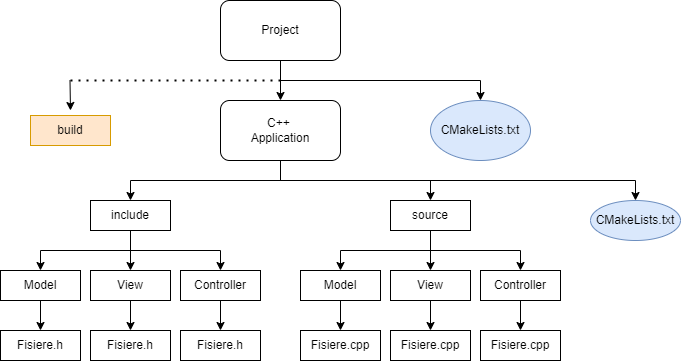
\includegraphics[width=0.8\linewidth]{structura_cmake.png}
  \caption{Structura directorului surs\u{a} al proiectului principal.}
  \label{fig:structura_cmake}
\end{figure}


\^{I}n figura \ref{fig:structura_cmake} este evidențiat\u{a} structura directorului surs\u{a} al proiectului, precum și utilizarea fișierului "CMakeLists.txt". Dup\u{a} ce proiectul este generat si configurat, se creeaz\u{a} directorul "build", unde vor fi prezente toate informațiile necesare rul\u{a}rii proiectului.

\section{Detecția placuțelor de \^{i}nmatriculare folosind OpenCV}

\subsection{Preprocesarea imaginii}
\subsubsection{Redimensionarea imaginii}
\subsubsection{Conversia imaginii in grayscale}
\subsubsection{Reducerea zgomotului}
\subsubsection{Operatia de Opening}
\subsubsection{Substracting}
\subsubsection{Thresholding}

\subsection{Postprocesarea imaginii}

\subsection{Rezultate}

\newpage

\section{Detecția placuțelor de \^{i}nmatriculare folosind rețele neurale convoluționale}

\subsection{Setul de imagini utilizat}
\subsection{Antrenarea modelului}
\subsection{Interferența in C++}

\subsection{Rezultate}

\section{Recunoașterea caracterelor din placuța de \^{i}nmatriculare}

\subsection{Preprocesarea imaginii}
\subsubsection{Undistortioning}
\subsubsection{Skew Correction}

\subsection{Rezultate}

\section{Modelarea entităților}

\section{Arhitectura aplicațiilor}

\section{Prezentarea aplicației C++}

\section{Prezentarea aplicației Web}

\section{Securitate}

\section{Concluzii și dezvoltări ulterioare}

\end{document}